
Bộ suy hao thụ động là thiết bị chuyên dụng để giảm cường độ tín hiệu từ nguồn đến thiết bị tiêu thụ mà không gây tác động tiêu cực đến sự ổn định của mạch chính. Nguyên lý hoạt động cốt lõi của bộ này nằm ở việc thiết kế sao cho tổng điện trở tương đương của mạng suy hao khi kết nối với thiết bị điện phải bằng đúng điện trở đi vào từ nguồn phát. Việc đảm bảo sự tương thích này giúp tối ưu hóa quá trình truyền dẫn và triệt tiêu các phản xạ năng lượng không mong muốn. 
\subsection*{Mạch suy hao T}
Để minh họa, ta xét một mạch điện gồm ba phần: 
\begin{itemize}
    \item (1): mạch nguồn vào gồm nguồn điện và điện trở bảo vệ $R_S$; 
    \item (2): mạch suy hao dạng chữ T gồm các điện trở $R_1$, $R_2$ và $R_3$; 
    \item (3): mạch ra gồm tải là một bóng đèn có điện trở $R_L$.
\end{itemize}

 Ở đây, điện trở tương đương của mạng suy hao sẽ là $R_{(2)(3)}$, điện trở đi vào từ nguồn là $R_{(1)}$.

\begin{figure}[htbp]
    \centering
    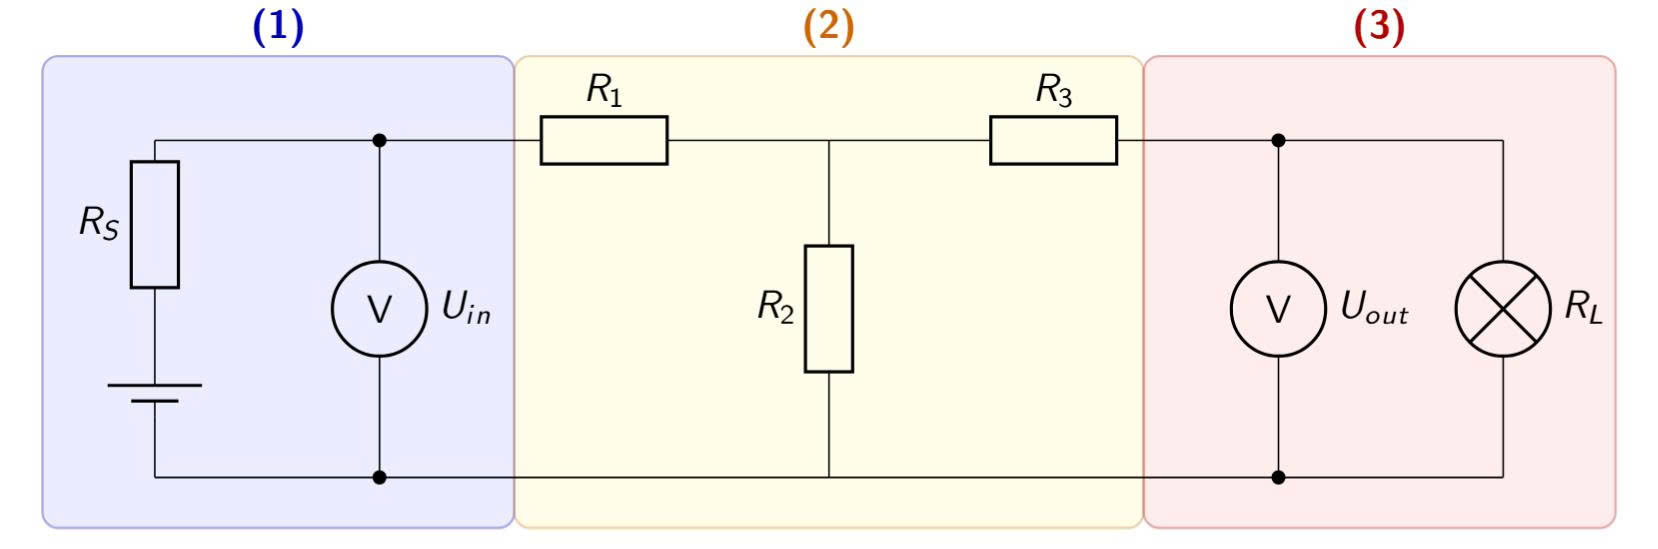
\includegraphics[width=1\textwidth]{Problem_3/Image/P3_I1.png}
    \caption{Mạch suy hao T}
\end{figure}

Ban đầu giá trị $R_S$ = $R_L$ = 50 \si{\ohm}, đặt mạch nguồn (1) và mạch ra (3) vào hai bên mạch (2), thực hiện các yêu cầu sau:

\begin{enumerate}[label=(\alph*)]
    \item  Chứng minh khi thay đổi vị trí của hai mạch (1) và (3), giá trị \(U_{out}\) ở mạch (3) vẫn không đổi.
    \item Tìm giá trị điện trở \(R_1\), \(R_2\), \(R_3\) để ta đạt được độ suy hao giữa công suất tại thiết bị điện so với điện trở nguồn là $10\%$
    \item Bây giờ thay đổi giá trị của $R_S$ = 100 \si{\ohm}, để độ suy hao không đổi thì các giá trị mới của $R_1$, $R_2$, $R_3$ là bao nhiêu?
\end{enumerate}
\newpage

\subsection*{Mạch suy hao T-Bridged}
Bộ suy hao T-Bridged là một biến thể khác của bộ suy hao T đối xứng tiêu chuẩn. Để minh họa, ta xét một mạch điện gồm 3 phần:

\begin{itemize}
    \item (1): mạch nguồn vào gồm nguồn điện và điện trở bảo vệ $R_{S}$
    \item (2): mạch suy hao dạng chữ T gồm các điện trở $R_{1}$, $R_{2}$, $R_{3}$ và $R_{4}$
    \item (3): mạch ra gồm tải là một bóng đèn có điện trở $R_L$.
\end{itemize}

\begin{figure}[htbp]
    \centering
    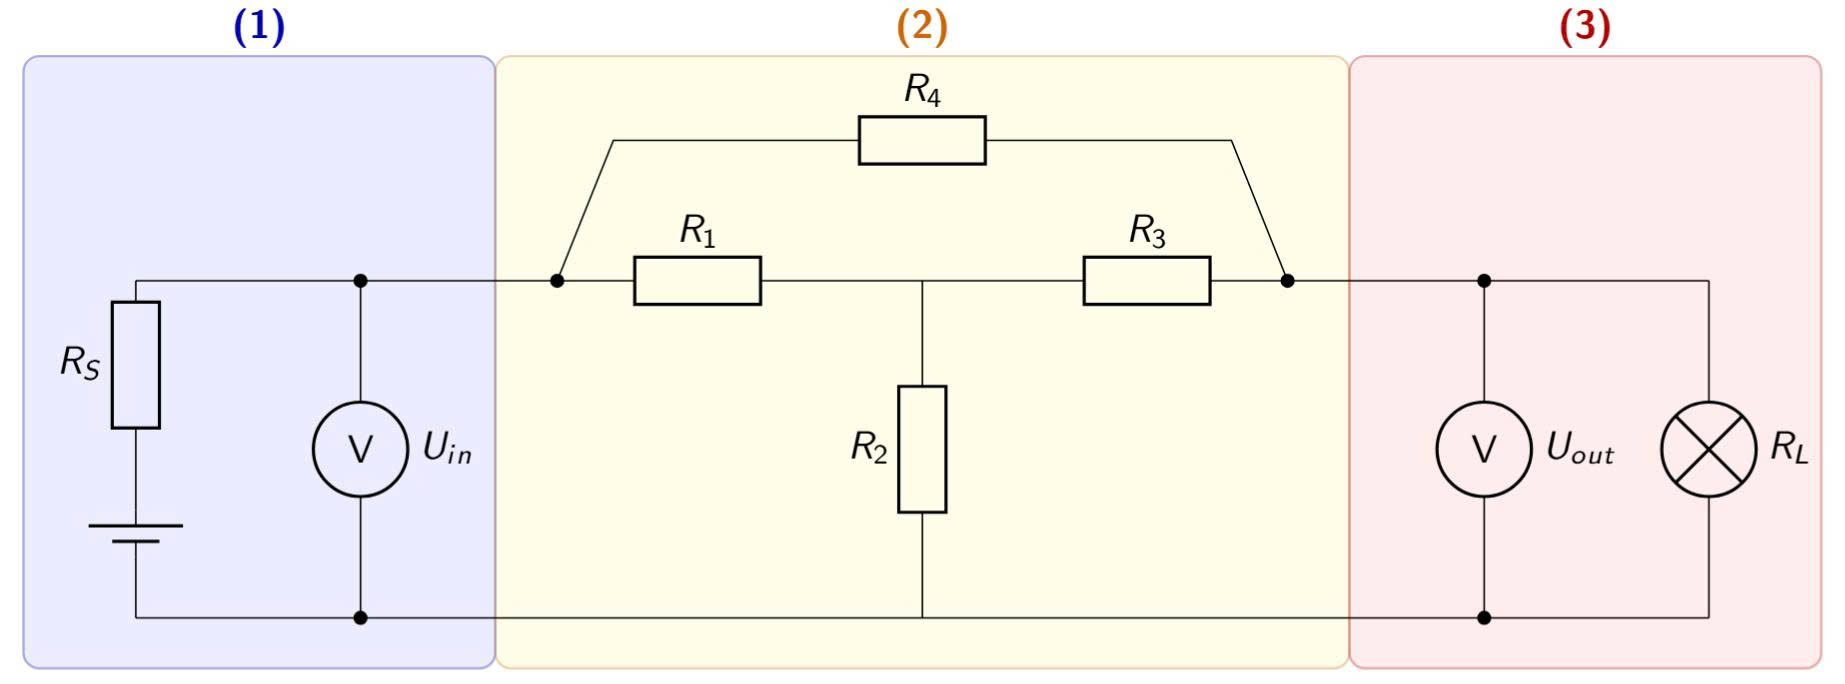
\includegraphics[width=0.8\textwidth]{Problem_3/Image/P3_I2.png}
    \caption{Mạch suy hao T-bridged}
\end{figure}

Tương tự như phần 1, $R_S$ = $R_L$ = 50 \si{\ohm}, đặt mạch nguồn (1) và mạch ra (3) vào hai bên mạch (2):

\begin{enumerate}[label=(\alph*)]
\addtocounter{enumi}{3}
    \item Hãy tìm giá trị điện trở $R_2$, $R_4$ để ta đạt được độ suy hao giữa công suất tại thiết bị điện so với điện trở nguồn là $10\%$.
    \item Biến trở đôi (dual-gang potentiometer) là linh kiện gồm hai biến trở được ghép cơ khí với nhau, cho phép hai giá trị điện trở thay đổi đồng thời theo từng nấc định trước. Dựa trên đặc điểm đó, hãy giải thích cách hoạt động của hai mạch đã nêu và so sánh khả năng của chúng trong việc thay đổi độ suy hao theo các mức rời rạc như 2\%; 4\%; 6\% hoặc 1\%; 3\%; 5\%. Trong mỗi nấc, hai giá trị điện trở phải thỏa mãn một quan hệ xác định để bảo đảm độ suy hao đạt đúng mức yêu cầu.
\end{enumerate}